\begin{figure*}[!t]
\centering
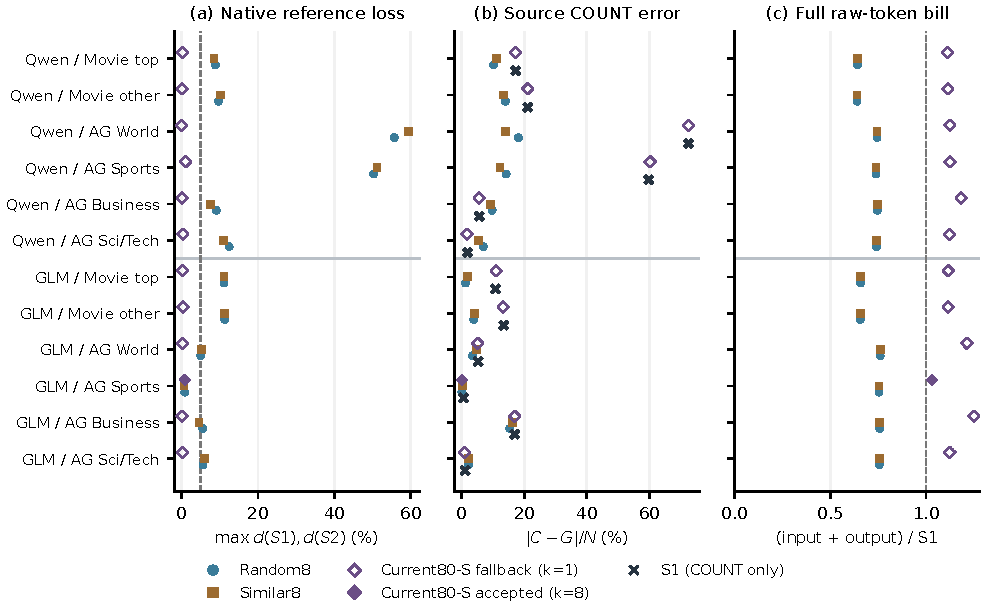
\includegraphics[width=\textwidth]{primary_execution_readouts.pdf}
\caption{All 12 primary configurations ($N=2,048$, cache ON), grouped by model. From left to right: the 0--5\% detail and full range of maximum disagreement with S1/S2; absolute source COUNT error divided by $N$; and complete input-plus-output tokens divided by S1. Smaller values are better. Dashed lines mark the 5\% reference threshold and unit cost. The two fidelity panels show the same measurements at different scales. Hollow diamonds denote fresh singleton fallback; only the filled diamond is an accepted batch. Crosses show S1's source COUNT error.}
\label{fig:primary}
\end{figure*}
